\section{\texttt{rpanel}}

\subsection{Descrição}

% ----------------------------------------------------------------------

\begin{frame}

  \texttt{rpanel} fornece um conjunto de funções para criar interfaces
  gráficas simples para controlar funções do R. Além destas, o pacote
  tem funções para interfaces específicas chamadas de \emph{cartoons}. É
  baseado em Tcl/Tk.

  \begin{itemize}
  \item Autores: Bowman, Bowman, Gibson and Crawford
  \item Lançamento: 21-Aug-2006
  \item Versão: 1.1-3
  \item URL:
    \url{http://cran.r-project.org/web/packages/rpanel/index.html}
  \end{itemize}

\end{frame}

% ----------------------------------------------------------------------

\subsection{Como usar}

\frame{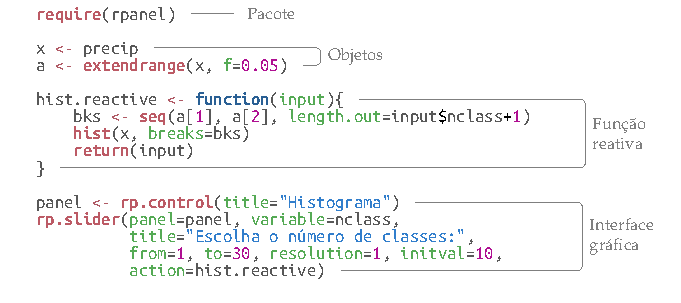
\includegraphics{./tikz/hist_slider_rpanel-1.pdf}}
\frame{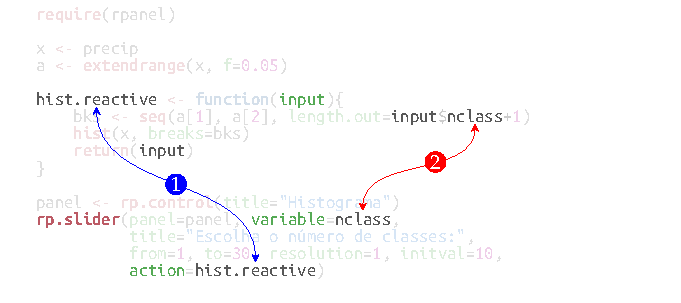
\includegraphics{./tikz/hist_slider_rpanel-2.pdf}}

\frame{
  \begin{center}
    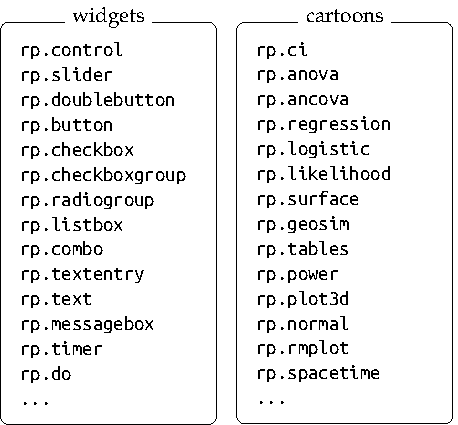
\includegraphics{./tikz/rpanel_fun.pdf}
  \end{center}
}

% ----------------------------------------------------------------------

\subsection{Exemplos}

\begin{frame}
  Praticando:
  \begin{enumerate}
  \item \href{run:../rpanel/rpanel.html}{Galeria rpanel iguir2}
  \end{enumerate}

  \vspace{0.5cm} Algumas aplicações com o rpanel:
  \begin{itemize}
  \item \href{http://www.stats.gla.ac.uk/~adrian/rpanel/}{Galeria do
      autor}
  \item \href{http://www.r-bloggers.com/?s=rpanel}{Busca no R Bloggers}
  \end{itemize}

\end{frame}

\begin{frame}

  Alguns pacotes com GUI baseadas em \texttt{rpanel}:
  \begin{itemize}
  \item
    \href{http://cran.r-project.org/web/packages/GUIDE/index.html}{\texttt{GUIDE}}
  \item
    \href{http://cran.r-project.org/web/packages/MDSGUI/index.html}{\texttt{MDSGUI}}
  \item
    \href{http://cran.r-project.org/web/packages/RVideoPoker/index.html}{\texttt{RVideoPoker}}
  \item
    \href{https://github.com/walmes/wzRfun/blob/master/R/rp.nls.R}{\texttt{wzRfun::rp.nls}}
    (\href{run:./images/rp-nls.gif}{abrir gif}).
  \item \ldots
  \end{itemize}

\end{frame}
